\documentclass{beamer}
\mode<presentation>{\usetheme{Frankfurt}}

\usepackage[english]{babel}
\usepackage[utf8]{inputenc}
\usepackage{times}
\usepackage[T1]{fontenc}

\usepackage{amsmath}
\usepackage[all]{xy}

\title{Text Surgery with vi}
\author{Nicholas C.~Spinale}
\institute{DevX \\ Carleton College}
\date{May 14^{th}, 2014}

\pgfdeclareimage[height=1cm]{thelogo}{devx-logo.png}
\logo{\pgfuseimage{thelogo}}

\AtBeginSubsection
    {
    \begin{frame}<beamer>{Outline}
        \tableofcontents[currentsubsection]
    \end{frame}
    }

\begin{document}

            \begin{frame}
            \titlepage
            \end{frame}

    \section*{Introduction}

            \begin{frame}{Introduction}
                \begin{center}
                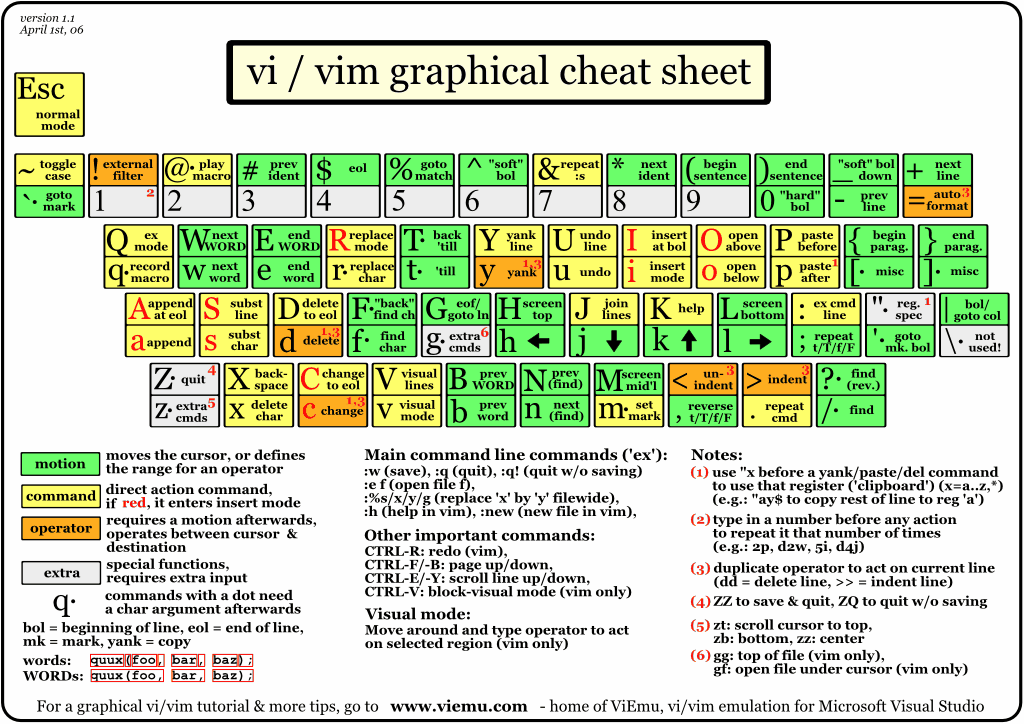
\includegraphics[width = 9.5cm, height = 7cm]{vi_vim_cheat_sheet.png}
                \end{center}
            \end{frame}

            \begin{frame}{My Plan}
            \tableofcontents
            \end{frame}

    \section{Background}

        \subsection{History}

            \begin{frame}{History}
                \begin{columns}[c]
                    \column{.5\textwidth}
                    Evolution of line editors
                    \begin{itemize}
                        \item 1971: ed at AT\&T
                        \item 1976: ex 0.1 by Bill Joy
                        \item 1979: ex 2.0/vi
                    \end{itemize}
                    \column{.4\textwidth}
                    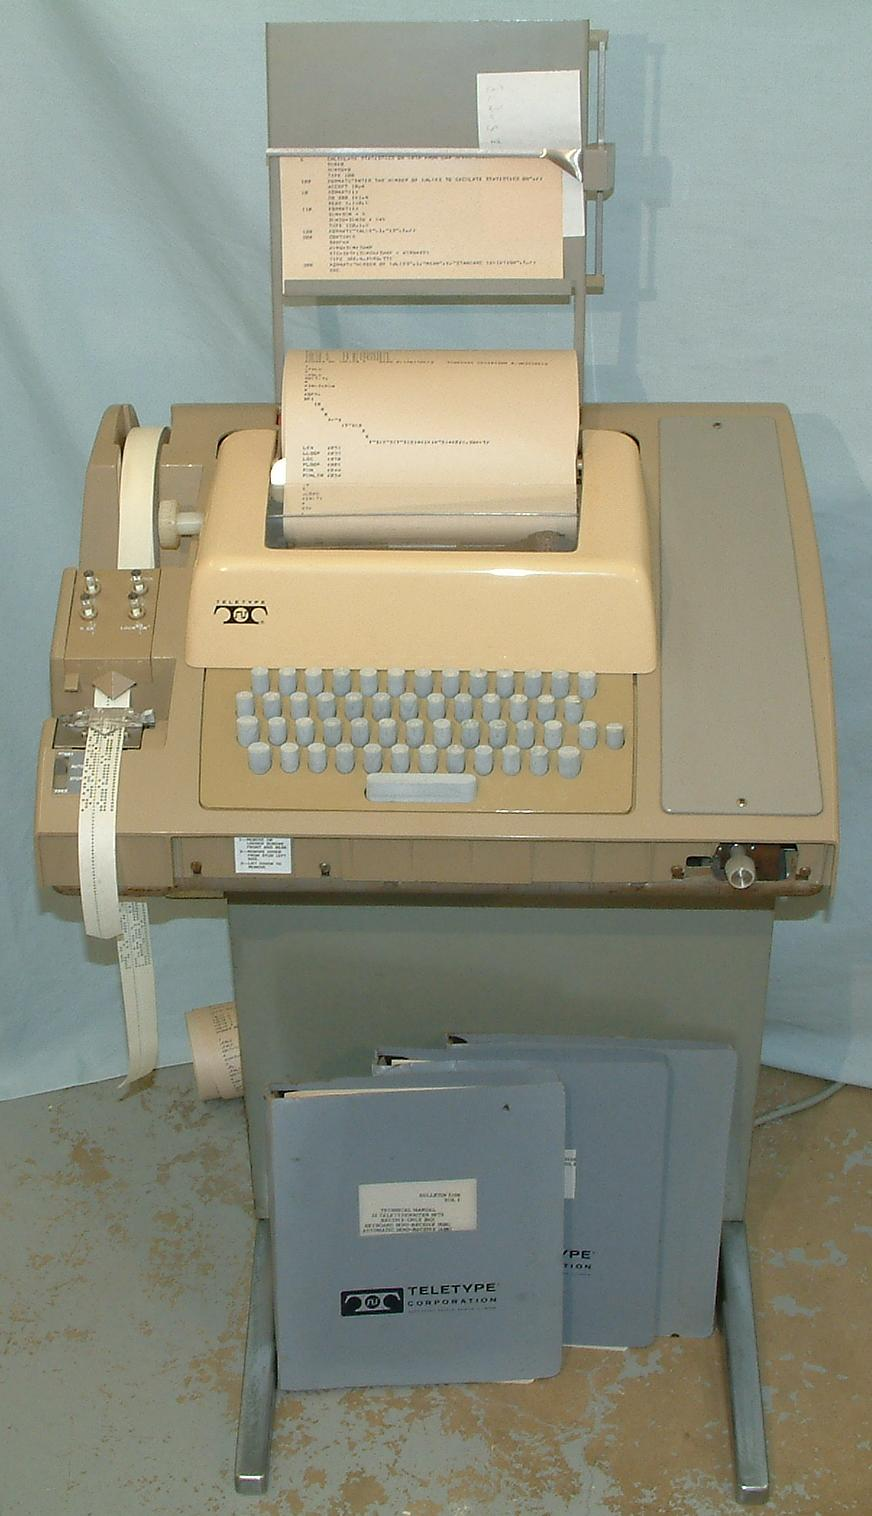
\includegraphics[height = 6cm]{teletype.jpg}
                \end{columns}
            \end{frame}

        \subsection{The vi Utility}

            \begin{frame}{The vi Utility}
                \texttt{vi [-rR] [-c command] [-t tagstring] [-w size] [file...]}
            \end{frame}

    \section{How to vi}

        \subsection{General Principles}

            \begin{frame}{wut is editor}
                \pause
                At the very least, it allows a user to
                \begin{itemize}
                    \pause
                    \item Load state of system into internal state
                    \pause
                    \item Modify internal state
                    \begin{itemize}
                        \pause
                        \item Buffers
                        \pause
                        \begin{itemize}
                            \item Contents
                            \item Position of cursor
                            \item Positions of other markers
                        \end{itemize}
                        \pause
                        \item Registers
                        \pause
                        \item Layout of buffers
                    \end{itemize}
                    \pause
                    \item Apply changes in internal state to system
                \end{itemize}
            \end{frame}

            \begin{frame}{A Clever Approach}
                Most editors: Key combinations \\~\\
                \pause
                vi: Modal editing/key sequences
            \end{frame}

        \subsection{Command Structure}

            \begin{frame}{Nouns}
                By themselves, they are considered 'motions'
                \begin{table}
                    \centering
                    \begin{tabular}{r|p{7cm}}
                        Left/down/up/right & \texttt{h/j/k/l} \\[.3cm]
                        Beginning of next word/Word & \texttt{w/W} \\[.3cm]
                        Beginning of last word/Word & \texttt{b/B} \\[.3cm]
                        Next/last occurence of \texttt{x} & \texttt{f/Fx} \\[.3cm]
                        Beginning/end of line & \texttt{\textasciicircum /\$ } \\[.3cm]
                        Next/last occurence of current word & \texttt{\#/*} \\
                    \end{tabular}
                \end{table}
                Numbers are adjectives
            \end{frame}

            \begin{frame}{Verbs}
            \end{frame}

            \begin{frame}{Visual Mode}
            \end{frame}

            \begin{frame}{Ex Commands}
            \end{frame}

            \begin{frame}{The Rest}
                Scrolling \\
                ZZ \\
                . \\
                etc
            \end{frame}

        \subsection{Registers}

            \begin{frame}{Registers}
                Named variables that store strings \\~\\
                Cut/copy to them \\
                Record them \\~\\
                Paste from them \\
                Play them
            \end{frame}

            \begin{frame}{The Art of Macros}
                Stay abstract. \pause Practice. \pause That is all.
            \end{frame}

            \begin{frame}{vi Golf}
                \texttt{i1<esc>qqyyp<c-a>q98@qqqcc Buzz<esc>5-q19@q2-qqciwFizz<esc>3+0q32@q}
            \end{frame}

    \section{Modern vi}

        \subsection{Vim}

            \begin{frame}{vi Improved}
                Ubiquitous \\~\\
                Compatability mode \\~\\
                Improvements
                \begin{itemize}
                    \item Aesthetics
                    \item Much more custmizability (including aesthetics...)
                    \item GUI mode
                \end{itemize}
            \end{frame}

            \begin{frame}{VimScript}
                There are TONS of plugins \\~\\
                Examples
                \begin{itemize}
                    \item Commentary
                    \item Tablizarize
                    \item Nerdtree
                    \item Ctrl-P
                \end{itemize}
            \end{frame}

        \subsection{Comparison to Other Editors}

            \begin{frame}{Emacs}
                \begin{center}
                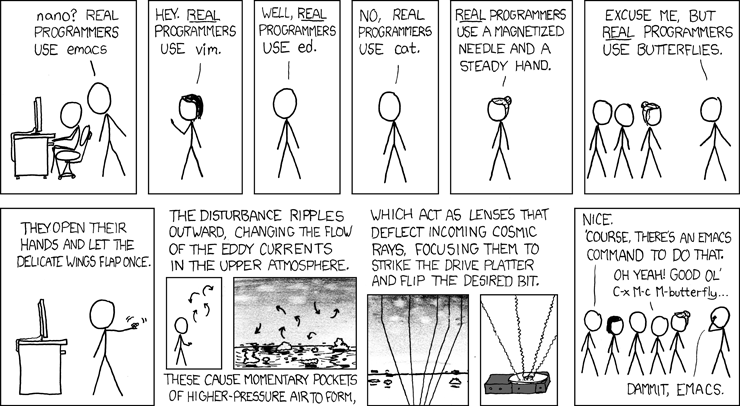
\includegraphics[width = 9.5cm, height = 5cm]{real_programmers.png}
                \end{center}
            \end{frame}

            \begin{frame}{IDE's}
                Pro: stay in terminal (seamlessly integrates with tmux, screen, etc) \\~\\
                \pause
                Con: learning curve
            \end{frame}

    \section*{Conclusion}

            \begin{frame}{Conclusion}
                \begin{center}
                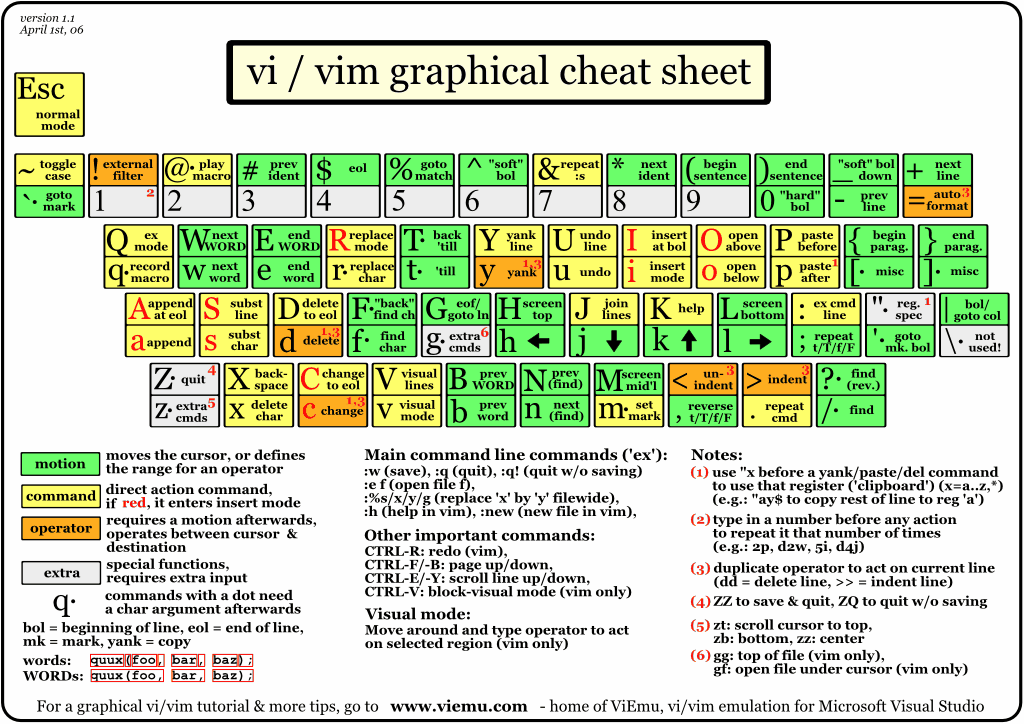
\includegraphics[width = 9.5cm, height = 7cm]{vi_vim_cheat_sheet.png}
                \end{center}
            \end{frame}


            \begin{frame}{Further Learning}
                How to continue learning
                \begin{itemize}
                    \item Cheatsheets (a few commands at a time)
                    \item VimDoc
                    \item VimCasts
                    \pause
                    \item Me \pause (I love talking about vim)
                \end{itemize}
            \end{frame}

            \begin{frame}{Questions?}
                \center{?}
            \end{frame}

\end{document}

% \begin{document}

%             \begin{frame}
%             \titlepage
%             \end{frame}

%     \section*{Introduction}

%             \begin{frame}{Introduction}
%                 Plan
%                 \begin{itemize}
%                     \item Vi's history as an editor
%                     \item The philosophy behind its design
%                     \item How to harness its power
%                     \item \emph{V}i \emph{IM}proved
%                 \end{itemize}
%                 Goals
%                 \begin{itemize}
%                     \item A foundation for learning
%                     \item Comfort with basic functions
%                 \end{itemize}
%             \end{frame}

%             \begin{frame}{My Plan}
%             \textbf{My message:} blindfolded solving does \emph{NOT} necessarily involve cheating, \emph{NOR} a photographic memory \\[.4cm]
%             \tableofcontents
%             \end{frame}

%     \section{What is Vi?}

%         \subsection{Background}

%             \begin{frame}{The Big Picture}
%                 \begin{itemize}
%                     \item Mathematical Objects
%                     \begin{itemize}
%                         \item Sets
%                         \item Functions
%                         \item Relations
%                         \item Quantities
%                     \end{itemize}
%                     \item Mathematics Structure: a set and one more more relevant objects
%                     \item Axioms define structures of particular interest to allow for generalizations
%                     \item Group Theory is the study of one such structure
%                 \end{itemize}
%             \end{frame}

%         \subsection{What is a Group?}

%             \begin{frame}{What is a Group?}
%                  For set \(G\) and binary operator \, \(*:G \, x \, G \to G\) \\
%                 \((G,*)\) is a group if, for any \(a,b,c \in G\)
%                 \begin{table}
%                     \centering
%                     \begin{tabular}{r|p{7cm}}
%                         Closure & \(a*b \in G\) \\[.3cm]
%                         Associativety & \((a*b)*c = a*(b*c)\) \\[.3cm]
%                         Identity & There exists some \(e \in G\) such that, for all \(g \in G, \, e*g = g*e = g\) \\[.3cm]
%                         Inverse & For all \(g \in G\), there exists some \(g^{-1}\) such that \(g*g^{-1} = g^{-1}*g = e\) \\
%                     \end{tabular}
%                 \end{table}
%             \end{frame}

%             \begin{frame}{An Example}
%                 \((\mathbb{R},*)\) \: The real numbers under multiplication
%                 \begin{table}
%                     \centering
%                     \begin{tabular}{r|p{7cm}}
%                         Closure & \(-6.7432*\frac{19}{3425} \in \mathbb{R}\) \\[.3cm]
%                         Associativety & \((6*2)*7 = 6*(2*7)\) \\[.3cm]
%                         Identity & 1*43 = 43*1= 43 \\[.3cm]
%                         Inverse & \(3*\frac{1}{3} = 1\) \\
%                     \end{tabular}
%                 \end{table}
%                 \emph{NOTE:} Not all groups are commutative!
%             \end{frame}

%     \section{A New Perspective on the Cube}

%             \begin{frame}{WE ARE READY!}
%                 \begin{center}
%                 \includegraphics[width = 7.2cm, height = 7.5cm]{thecube.png}
%                 \end{center}
%             \end{frame}

%         \subsection{Necessary Info}

%             \begin{frame}{Some Important Notes}
%                 We will never move the centers! \\[.3cm]
%                 Groups of stickers belong to pieces, so \\[.1cm]
%                 \( \quad \quad \) Corner stickers and edge stickers remain as such \\[.1cm]
%                 \( \quad \quad \) Each sticker has \emph{EXACTLY 1} correct position \\[.3cm]
%                 States vs. effects \\[.4cm]
%                 There are \( 18 = 6*3 \) legal primative effects
%                 \[R,L,U,D,F,B\]
%                 \[R^{-1},L^{-1},U^{-1},D^{-1},F^{-1},B^{-1}\]
%                 \[R^{2},L^{2},U^{2},D^{2},F^{2},B^{2}\]
%             \end{frame}

%         \subsection{The Cube Group}

%             \begin{frame}{The Cube Group}
%                 Let set \(X_{C}\) contain the 24 corner sticker locations\\
%                 Let set \(X_{E}\) contain the 24 edge sticker locations\\[.3cm]
%                 Consider a pair of bijective maps ("re-arrangements")
%                 \[ \sigma : X_C \to X_C \text{  and  } \tau : X_E \to X_E \]  \\[.2cm]
%                 \( \sigma \) assigns a new corner location to each corner location \\
%                 \( \tau \) assigns a new edge location to each edge location \\[.2cm]
%                 All elements of \( G = \, <R,L,U,D,F,B> \), \\
%                 the set of legal effects on a state of the cube, \\
%                 are composed of one such \( \sigma \) and one such \( \tau \)
%                 \[ G = \{ \, (\sigma , \tau) \,| \,\sigma \in A(X_C), \tau \in A(X_C) \,\} \]
%             \end{frame}

%             \begin{frame}{Example: \( F = (\sigma_F ,\tau_F) \)}
%                 \begin{columns}[c]
%                     \column{.7\textwidth}
%                     \includegraphics[width = 8cm]{FPERM.png} \\
%                     \( \sigma_F \scriptstyle = (\,I\,J\,K\,L\,)\,(\,D\,M\,V\,G\,)\,(\,C\,P\,U\,F\,) = (\,I\,J\,K\,L\,) = \dots \) \\
%                     \( \tau_F \scriptstyle = (\,I\,J\,K\,L\,)\,(\,C\,P\,U\,F\,) = (\,I\,J\,K\,L\,) = (\,C\,P\,U\,F\,) \)
%                     \column{.3\textwidth}
%                     \includegraphics[height = 7cm]{fpermtable.png}
%                 \end{columns}
%             \end{frame}

%             \begin{frame}{The Cube Group: \( (g,*) \)}
%                 \(G\) is a group under "\(*\)" (composition)
%                 \[ a = (\sigma_1,\tau_1), b = (\sigma_2,\tau_2) \implies a*b = (\sigma_1 \circ \sigma_2, \tau_1 \circ \tau_2) \]
%                 \[ (\upsilon_{1} \circ \upsilon_{2}) (a) = \upsilon_{2} (\upsilon_{1} (a))\] \\
%                 \begin{table}
%                     \centering
%                     \begin{tabular}{r|p{7cm}}
%                         Closure & \( a,b \in G \implies a*b \in G \) \\[.3cm]
%                         Associativety & \( (a*b)*c = a*(b*c) \) \\[.3cm]
%                         Identity & Let \((e,e)\) map every location to itself \\[.3cm]
%                         Inverse & \(a = (\sigma, \tau) \implies a^{-1} = (\sigma^{-1}, \tau^{-1}) \) \\
%                     \end{tabular}
%                 \end{table}
%             \end{frame}

%     \section{Blindfolded Cubing}

%         \subsection{The General Strategy}

%             \begin{frame}{The General Strategy}
%                 Phase 1: Memorization \\[.1cm]
%                 \quad \quad After observing cube scrambled by \( s = (\sigma_s,\tau_s) \)  \\
%                 \quad \quad find effect \( m = (\sigma_m,\tau_m) \) \\
%                 \quad \quad such that \( s * m = (\sigma_s \circ \sigma_m, \tau_s \circ \tau_m) = (e,e) \) \\[.5cm]
%             \pause
%                 Phase 2: Execution \\
%                 \begin{itemize}
%                     \item \emph{SIMPLIFY}: make small alterations\\
%                     \item Group theory tells us that smallest are 3-cycles of either corners or edges\\
%                     \item For \( \sigma_m \) and \( \tau_m \) seperately, \\
%                         use 3-cycles to reduce each permutation to \\
%                         either \(e\) or a double transposition
%                     \item If necessary, deal with parity \\[.3cm]
%                 \end{itemize}
%             \end{frame}

%         \subsection{Execution Techniques}

%             \begin{frame}{Execution Techniques}
%                 Creating 3-cycles \\[.2cm]
%                 \begin{itemize}
%                     \item Commutators: \quad \( aba^{-1}b^{-1} \) \quad denoted \( [\,a\,;b\,]\)
%                     \item Conjugates: \quad \( aba^{-1} \) \quad denoted \( <a\,;b> \) \\[.7cm]
%                 \end{itemize}
%                 Dealing with Parity
%             \end{frame}

%             \begin{frame}{Easy-ization}
%                 Ways to make the above approach practical for a human \\[.2cm]
%                 \begin{itemize}
%                     \item Buffer spots
%                     \item Stefan Pochmann
%                     \item M2 and R2 methods
%                     \item The classical approach
%                 \end{itemize}
%             \end{frame}

%     \section*{Conclusion}

%             \begin{frame}{Conclusion}
%                 Parting Words \\[.2cm]
%                 \begin{itemize}
%                     \item I can give you resources to learn more about group theory
%                     \item I can give you resources to learn more about the cube
%                     \item If enough people want to come, I can demonstrate a blindfolded solve
%                 \end{itemize}
%             \end{frame}

%             \begin{frame}{Thank You}
%                 \begin{center}
%                 \includegraphics[width = 7.2cm, height = 7.5cm]{thecube.png}
%                 \end{center}
%             \end{frame}

% \end{document}
